\documentclass{article}
\usepackage{graphicx}
\usepackage{IEEEtrantools}
\usepackage{amsmath}

\title{Solve $Z_1 = Z_2$ for $x_1$}
\author{Daniel Fishbein}

\begin{document}
\maketitle

\section{Given:}

\begin{figure}[h!]{
    \centering
    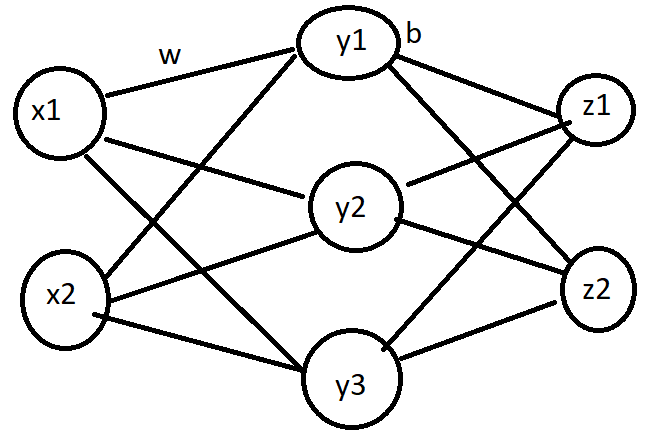
\includegraphics[width=0.5\linewidth]{Given_NN.png}
    \caption{Given Neural Net}\label{fig:NeuralNet}
    }
\end{figure}

\hbox{Figure~\ref{fig:NeuralNet} shows the given Neural Net that will be analysed.}

\vspace{5mm}

\hbox{$x_1, x_2$ are the input neurons}
\hbox{$[x]$ is the columnised vector notation of all "x" neurons of dimentions $1$X$x$}
\vspace{1mm}

\hbox{$y_1, y_2, y_3$ are the hidden layers neurons}
\hbox{$[y]$ is the columnised vector notation of all "y" neurons of dimentions $1$X$y$}
\vspace{1mm}

\hbox{$z_1, z_2$ are the output neurons}
\hbox{$[z]$ is the columnised vector notation of all "z" neurons of dimentions $1$X$z$}

\vspace{2mm}
\hbox{$w$ denotes a weight}
\hbox{$w_{y_1->z_2}$ denotes the weight from $y_1$ to $z_2$}
\hbox{$[w_1]$ is the columnised vector notation of all "$w_1$" weights of dimentions $y$X$x$}
\hbox{$[w_1] = [
    \begin{matrix}
        w_{11} w_{12} w_{13} ... w_{1x} \\
        :\\
        w_{ij}\\
        :\\
        w_{y1} w_{y2} w_{y3} ... w_{yx}
    \end{matrix}
]$}

\vspace{2mm}
\hbox{$[w_2]$ is the columnised vector notation of all "$w_2$" weights of dimentions $z$X$y$}
\hbox{$[w_2] = [
    \begin{matrix}
        w_{11} w_{12} w_{13} ... w_{1y} \\
        :\\
        w_{ij}\\
        :\\
        w_{z1} w_{z2} w_{z3} ... w_{zy}
    \end{matrix}
]$}


\vspace{4mm}
\hbox{$b$ deontes a bias}
\hbox{$b_{y_3}$ deontes the bias associated with neuron $y_3$}
\hbox{$[b_1]$ is the columnised vector notation of all "$b_1$" biases of dimentions $1$X$y$ }
\hbox{$[b_1] = [
    \begin{matrix}
        b_{11}\\
        b_{21}\\
        :\\
        b_{1y}
    \end{matrix}
]$}

\vspace{2mm}
\hbox{$[b_2]$ is the columnised vector notation of all "$b_2$" biases of dimentions $1$X$z$ }
\hbox{$[b_2] = [
    \begin{matrix}
        b_{11}\\
        b_{21}\\
        :\\
        b_{1z}
    \end{matrix}
]$}

\vspace{5mm}
\hbox{The input to a $y_i$ neuron will be denoted as:}
\hbox{$y_i = \sigma(w_{x_1->y_i} * x_1 + w_{x_2->y_i} * x_2 + b_{y_i} )$}
\hbox{OR in vector notation:}
\hbox{$[y] = \sigma([x][w_1] + [b_1])$}

\vspace{2mm}
\hbox{Where $\sigma(x) = \frac{1}{1+e^{-x}} = \frac{1}{1+\exp[-x]}$}

\vspace{5mm}
\hbox{The input to a $z_i$ neuron will be denoted as:}
\hbox{$z_i = \sigma(w_{y_1->z_i}*y_1 + w_{y_2->z_i}*y_2 + w_{y_3->z_i}*y_3 + b_{z_i} )$}
\hbox{OR in vector notation:}
\hbox{$[z] = \sigma([y][w_2] + [b_2])$}
\end{document}